\documentclass{article}
\usepackage{graphicx}
\usepackage{tikz}
\usetikzlibrary{positioning}

\title{Graph Theory and Network Analysis: \\
       Exploring Applications in Computer Science}
\author{Badger Code}
\date{\today}

\begin{document}
\maketitle

\section{Introduction}
Graph theory is a mathematical discipline that studies the properties and relationships of graphs, which consist of nodes (vertices) connected by edges. This paper explores the applications of graph theory in computer science, with a focus on social networks, computer networks, and routing algorithms. Graphs are used to model complex relationships and connectivity patterns in various real-world systems, and their analysis plays a pivotal role in understanding and optimizing network structures and algorithms.

\section{Graph Fundamentals}
Before delving into applications, let's establish some fundamental concepts in graph theory.

\subsection{Graph Definition}
A graph $G$ is a pair $(V, E)$, where $V$ is a set of vertices (nodes), and $E$ is a set of edges (connections). Each edge in $E$ is an unordered pair of vertices in $V$, representing a relationship or connectivity between them.

\subsection{Types of Graphs}
Graphs can be classified into various types based on their characteristics. Common types include:
\begin{itemize}
    \item \textbf{Undirected Graph:} Edges have no direction, and the order of vertices in an edge does not matter.
    \item \textbf{Directed Graph (Digraph):} Edges have a direction, represented by arrows, indicating a one-way relationship between vertices.
    \item \textbf{Weighted Graph:} Each edge has an associated weight, which can represent distance, cost, or any other relevant quantity.
    \item \textbf{Cyclic Graph:} Contains at least one cycle, where a cycle is a closed path of edges and vertices.
    \item \textbf{Acyclic Graph:} Contains no cycles.
\end{itemize}

\subsection{Graph Representation}
Graphs can be represented using various data structures, such as adjacency matrix or adjacency list. These representations impact the efficiency of graph algorithms.

\section{Applications in Social Networks}
Social networks are a prominent area where graph theory finds widespread application. Social networks model relationships between individuals or entities and provide insights into community structures and information dissemination.

\subsection{Friendship Graph}
In a social network, each user is represented as a node, and an edge exists between two nodes if the corresponding users are friends.

\begin{center}
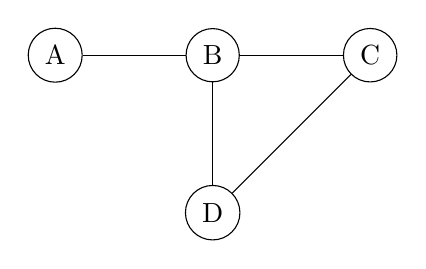
\begin{tikzpicture}
  \node[circle, draw] (A) at (0,0) {A};
  \node[circle, draw] (B) at (2,0) {B};
  \node[circle, draw] (C) at (4,0) {C};
  \node[circle, draw] (D) at (2,-2) {D};

  \draw (A) -- (B);
  \draw (B) -- (C);
  \draw (B) -- (D);
  \draw (C) -- (D);
\end{tikzpicture}
\end{center}

In the example above, users A, B, C, and D form a social network, where A is friends with B, B is friends with C and D, and C is friends with D.

\subsection{Community Detection}
Graph analysis techniques, such as clustering algorithms, can identify communities or groups of densely connected nodes in social networks.

\begin{center}
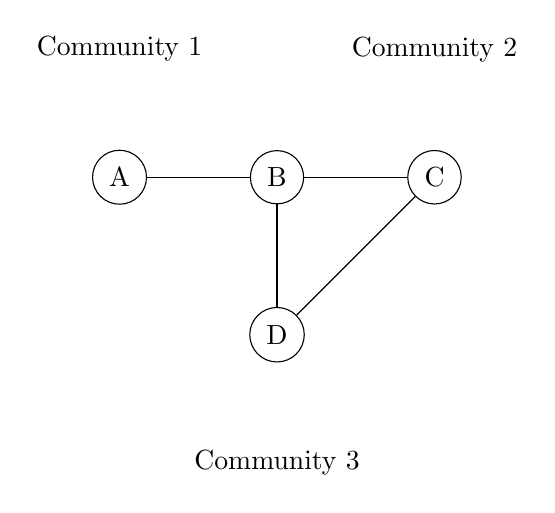
\begin{tikzpicture}
  \node[circle, draw] (A) at (0,0) {A};
  \node[circle, draw] (B) at (2,0) {B};
  \node[circle, draw] (C) at (4,0) {C};
  \node[circle, draw] (D) at (2,-2) {D};

  \draw (A) -- (B);
  \draw (B) -- (C);
  \draw (B) -- (D);
  \draw (C) -- (D);

  \node[draw=none, above=of A] {Community 1};
  \node[draw=none, above=of C] {Community 2};
  \node[draw=none, below=of D] {Community 3};
\end{tikzpicture}
\end{center}

In this example, the social network can be divided into three distinct communities.

\subsection{Information Diffusion}
Graphs model the spread of information in social networks. The study of viral marketing and influence maximization involves identifying influential nodes for efficient information dissemination.

\section{Applications in Computer Networks}
Graph theory is fundamental in computer networks for analyzing connectivity, optimizing routing, and understanding network topologies.

\subsection{Network Topology}
In computer networks, nodes represent devices (e.g., computers, routers), and edges represent physical or logical connections between them.

\begin{center}
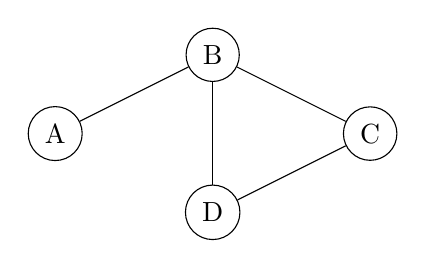
\begin{tikzpicture}
  \node[circle, draw] (A) at (0,0) {A};
  \node[circle, draw] (B) at (2,1) {B};
  \node[circle, draw] (C) at (4,0) {C};
  \node[circle, draw] (D) at (2,-1) {D};

  \draw (A) -- (B);
  \draw (B) -- (C);
  \draw (B) -- (D);
  \draw (C) -- (D);
\end{tikzpicture}
\end{center}

In this example, the nodes represent devices (A, B, C, D), and the edges represent the connections between them.

\subsection{Connectivity Analysis}
Graph theory helps analyze the connectivity of computer networks, determining if all nodes are reachable or if there are isolated components.

\subsection{Routing Algorithms}
Graph algorithms, such as Dijkstra's algorithm or the Bellman-Ford algorithm, are used to find the shortest path between nodes, crucial for routing packets efficiently in computer networks.

\begin{center}
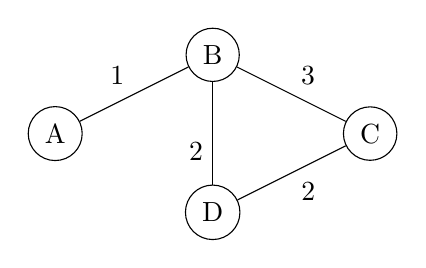
\begin{tikzpicture}
  \node[circle, draw] (A) at (0,0) {A};
  \node[circle, draw] (B) at (2,1) {B};
  \node[circle, draw] (C) at (4,0) {C};
  \node[circle, draw] (D) at (2,-1) {D};

  \draw (A) -- (B) node[midway, above left] {1};
  \draw (B) -- (C) node[midway, above right] {3};
  \draw (B) -- (D) node[midway, below left] {2};
  \draw (C) -- (D) node[midway, below right] {2};
\end{tikzpicture}
\end{center}

In this example, each edge is labeled with its respective weight. Dijkstra's algorithm can be used to find the shortest path between any pair of nodes.

\section{Applications in Routing Algorithms}
Routing algorithms are essential in computer networks to efficiently transfer data between nodes. Graph theory helps design and optimize these algorithms.

\subsection{Shortest Path Routing}
Shortest path algorithms, such as Dijkstra's algorithm and the Bellman-Ford algorithm, find the most efficient path between a source and destination node.

\subsection{Routing in Sensor Networks}
In wireless sensor networks, graph-based routing algorithms help transmit data from sensors to a central node or sink efficiently.

\subsection{Routing in the Internet}
Graph-based routing protocols, like OSPF (Open Shortest Path First) and BGP (Border Gateway Protocol), are used in the Internet's routing infrastructure to ensure efficient data delivery.

\section{Conclusion}
Graph theory's applications in computer science are far-reaching, from modeling social networks and analyzing their properties to optimizing computer networks' routing algorithms. The use of graph theory enables the efficient analysis and understanding of complex network structures and connectivity patterns. Its impact on computer science will continue to grow as technology advances, and more sophisticated graph algorithms are developed to tackle increasingly complex networks.

\end{document}